\newpage
\hypertarget{invertCard tex}{}
\subsection{Implementing invert}
\texHeader

\begin{itemize}

\item[$\blacktriangleright$] You're no longer an SDM beginner, so create a simple control flow with two patterns in \texttt{card.eclass} in the invert
method named \texttt{initializeTemp} and \texttt{swapVariable}. Don't forget to include a return statement (Fig.~\ref{fig:eclipse_invert}) !

\begin{figure}[htbp]
\begin{center}
  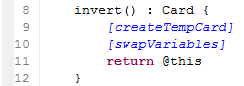
\includegraphics[width=0.4\textwidth]{eclipse_invertControlFlow}
  \caption{Control flow for \texttt{card.invert}}  
  \label{fig:eclipse_invert}
\end{center}
\end{figure}

\item[$\blacktriangleright$] Create \texttt{this} and \texttt{temp} \texttt{Card} variables in each pattern until your workspace resembles
Fig.~\ref{fig:invertPatternsDecs}.

\begin{figure}[htbp]
\begin{center}
  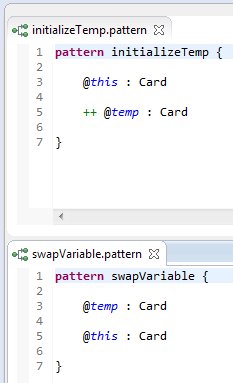
\includegraphics[width=0.4\textwidth]{eclipse_invertPatternDecs}
  \caption{Swapping the \texttt{card} values}  
  \label{fig:invertPatternsDecs}
\end{center}
\end{figure}

\item[$\blacktriangleright$] Notice that the binding operator on \texttt{temp} in \texttt{initializeTemp} is set to create! This is so that we actually
\emph{make} a new object, and not pattern match to an existing one in the model. It won't be persisted in the model afterwards which makes this truly a
\emph{temporary} variable.

\item[$\blacktriangleright$] Next, we need to declare four assignments within the \texttt{temp} and \texttt{card} rules, the first pair to assign the values to
\texttt{temp}, and the latter to actually switch the values. Your workspace should now resemble Fig.~\ref{fig:invertPatterns}.

\begin{figure}[htbp]
\begin{center}
  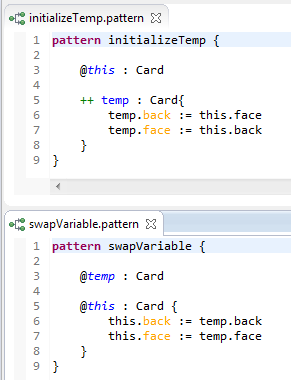
\includegraphics[width=0.5\textwidth]{eclipse_invertPatterns}
  \caption{Swapping the \texttt{card} values}  
  \label{fig:invertPatterns}
\end{center}
\end{figure}

\item[$\blacktriangleright$] Believe it or not, that's it! We recommend building at this point to confirm you have made no mistakes. To
see this method in the visual syntax, review Fig.~\ref{fig:sdm_invertComplete} in the previous section.

\end{itemize}
